
	\begin{subfigure}{0.25\textwidth}
	\centering
	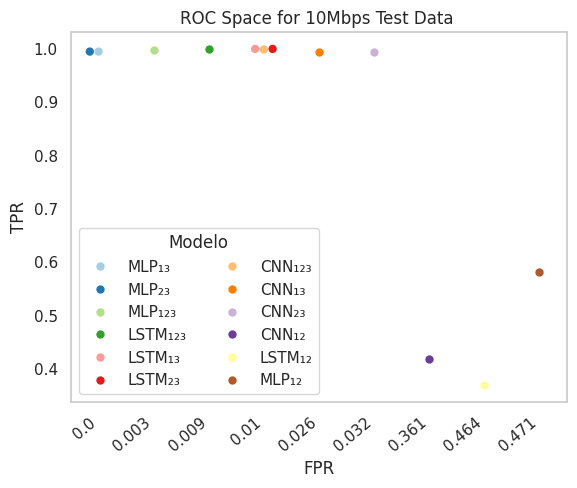
\includegraphics[width=1.0\textwidth]{./figs/ROC-Space-Test-Data-10Mbps.png}
	\caption{Lorem ipsum}
\end{subfigure}%
~ 
\begin{subfigure}{0.25\textwidth}
	\centering
	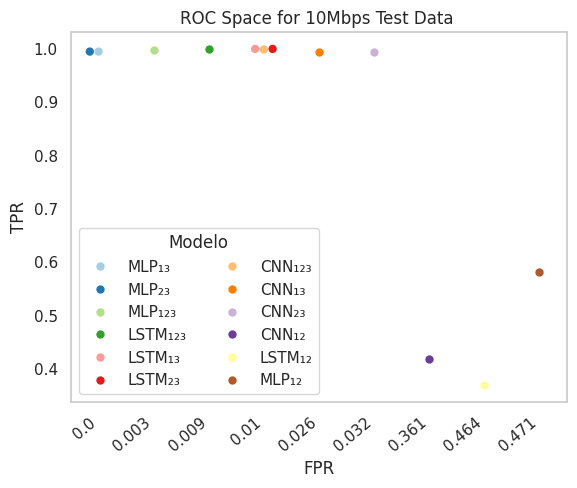
\includegraphics[width=1.0\textwidth]{./figs/ROC-Space-Test-Data-10Mbps.png}
	\caption{Lorem ipsum}
\end{subfigure}
~ 
\begin{subfigure}{0.25\textwidth}
	\centering
	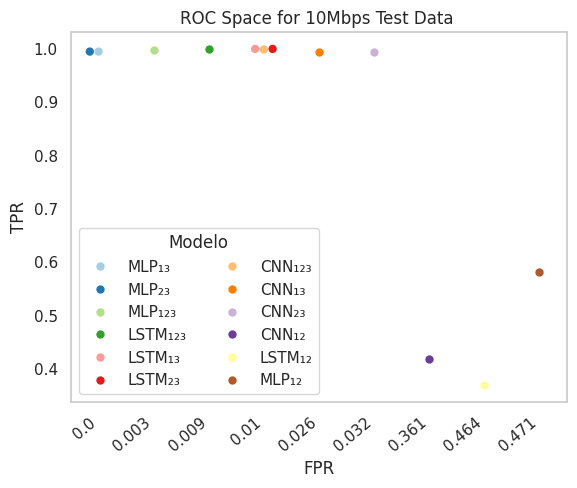
\includegraphics[width=1.0\textwidth]{./figs/ROC-Space-Test-Data-10Mbps.png}
	\caption{Lorem ipsum}
\end{subfigure}

\begin{subfigure}{0.25\textwidth}
	\centering
	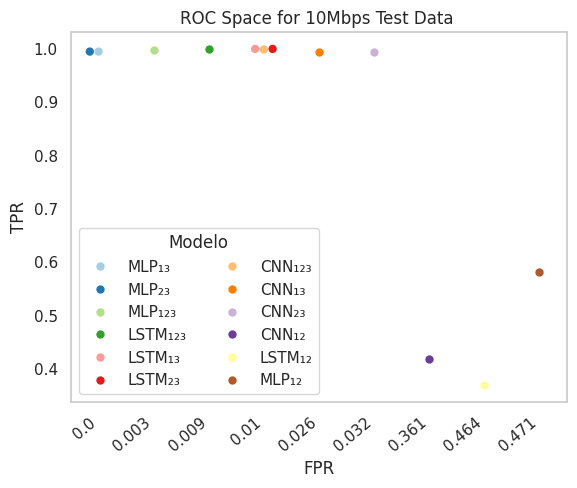
\includegraphics[width=1.0\textwidth]{./figs/ROC-Space-Test-Data-10Mbps.png}
	\caption{Lorem ipsum}
\end{subfigure}
~ 
\begin{subfigure}{0.25\textwidth}
	\centering
	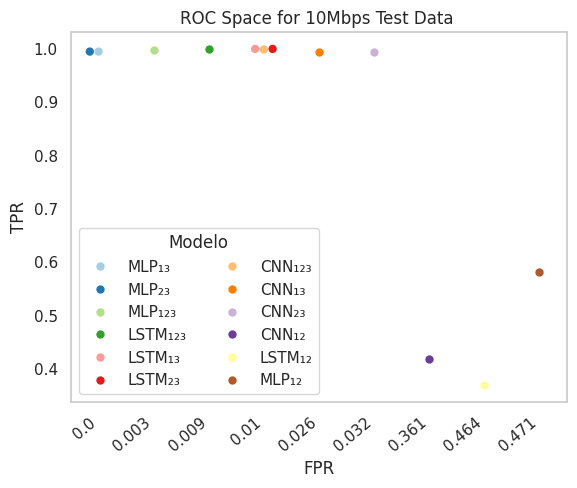
\includegraphics[width=1.0\textwidth]{./figs/ROC-Space-Test-Data-10Mbps.png}
	\caption{Lorem ipsum}
\end{subfigure}
~ 
\begin{subfigure}{0.25\textwidth}
	\centering
	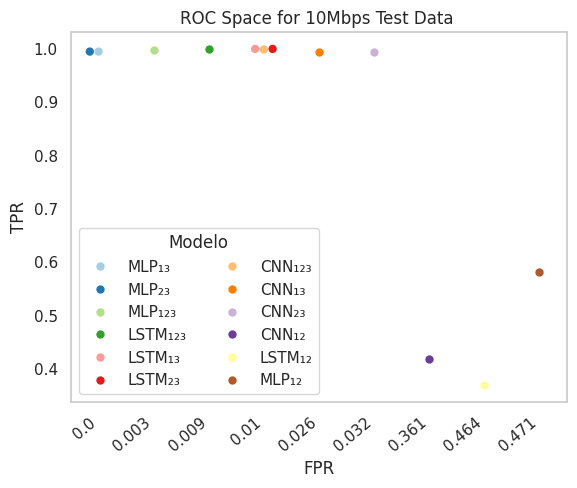
\includegraphics[width=1.0\textwidth]{./figs/ROC-Space-Test-Data-10Mbps.png}
	\caption{Lorem ipsum}
\end{subfigure}

\begin{subfigure}{0.25\textwidth}
	\centering
	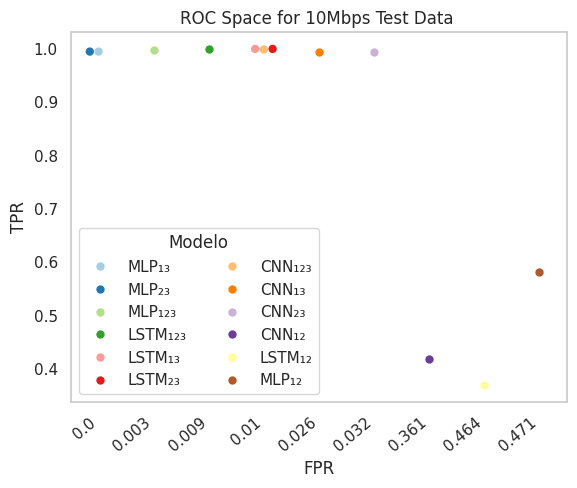
\includegraphics[width=1.0\textwidth]{./figs/ROC-Space-Test-Data-10Mbps.png}
	\caption{Lorem ipsum}
\end{subfigure}
~ 
\begin{subfigure}{0.25\textwidth}
	\centering
	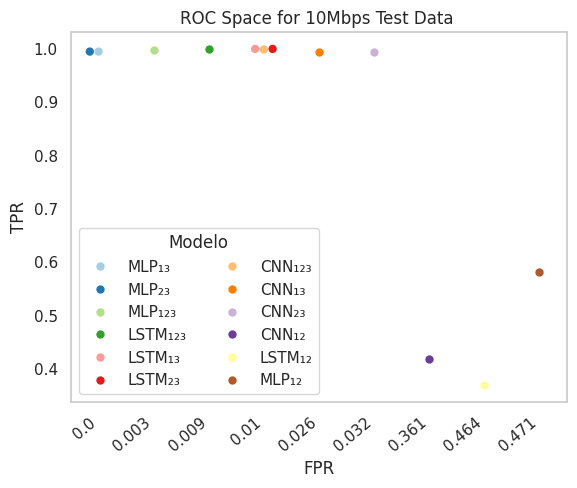
\includegraphics[width=1.0\textwidth]{./figs/ROC-Space-Test-Data-10Mbps.png}
	\caption{Lorem ipsum}
\end{subfigure}
~ 
\begin{subfigure}{0.25\textwidth}
	\centering
	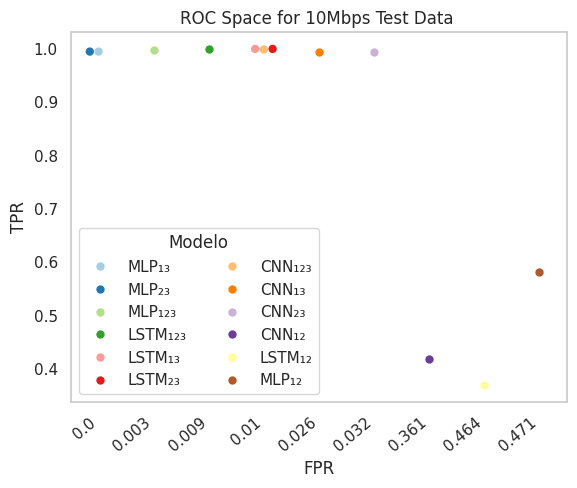
\includegraphics[width=1.0\textwidth]{./figs/ROC-Space-Test-Data-10Mbps.png}
	\caption{Lorem ipsum}
\end{subfigure}







\begingroup
\captionsetup[figure]{font=tiny}
\hfill
\begin{minipage}{0.1\textwidth}
	\centering
	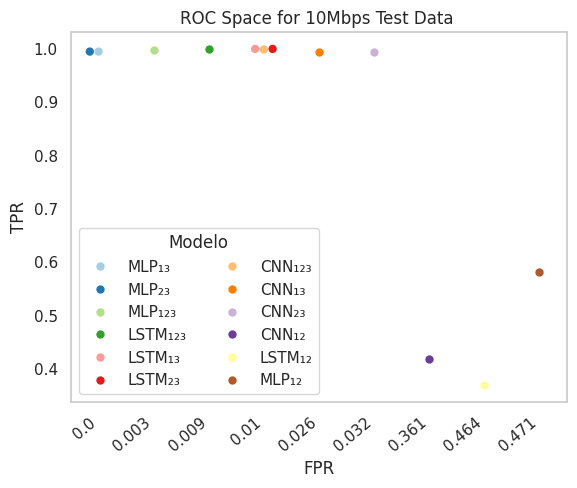
\includegraphics[width=1.0\textwidth]{./figs/ROC-Space-Test-Data-10Mbps.png}
	\captionof{figure}{ROC space test Data 10Mbps.}
	\label{fig:ROCDesempenhoteste10Mbps}	
\end{minipage}
%\hfill
\begin{minipage}{0.1\textwidth}
	\centering
	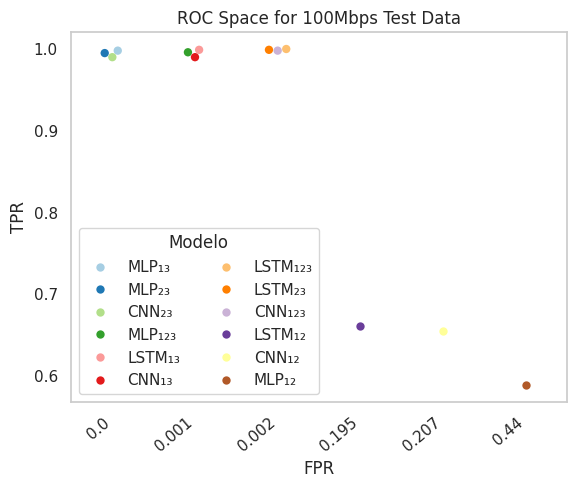
\includegraphics[width=1.0\textwidth]{./figs/ROC-Space-Test-Data-100Mbps.png}
	\captionof{figure}{ROC space test Data 100Mbps.}
	\label{fig:ROCDesempenhoteste100Mbps}	
\end{minipage}
%\hfill
%\\
%\\
%\hfill
\begin{minipage}{0.1\textwidth}
	\centering
	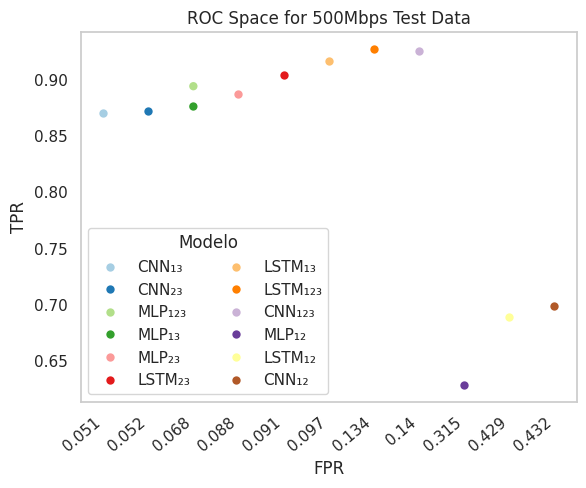
\includegraphics[width=1.0\textwidth]{./figs/ROC-Space-Test-Data-500Mbps.png}
	\captionof{figure}{ROC space test Data 500Mbps.}
	\label{fig:ROCDesempenhoteste500Mbps}	
\end{minipage}
%\hfill
\begin{minipage}{0.1\textwidth}
	\centering
	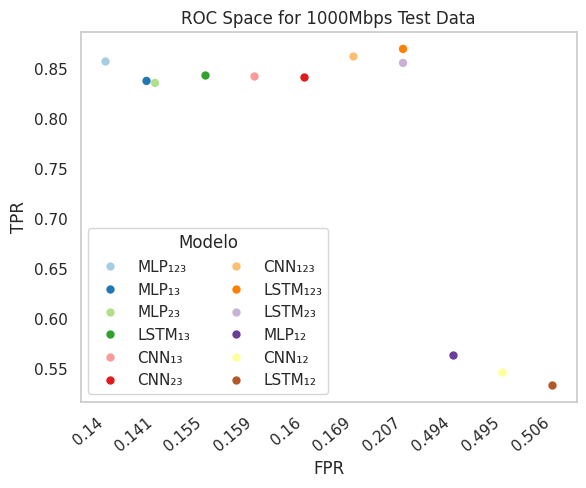
\includegraphics[width=1.0\textwidth]{./figs/ROC-Space-Test-Data-1000Mbps.png}
	\captionof{figure}{ROC space test Data 1000Mbps.}
	\label{fig:ROCDesempenhoteste1000Mbps}	
\end{minipage}
%\hfill
\begin{minipage}{0.1\textwidth}
	\centering
	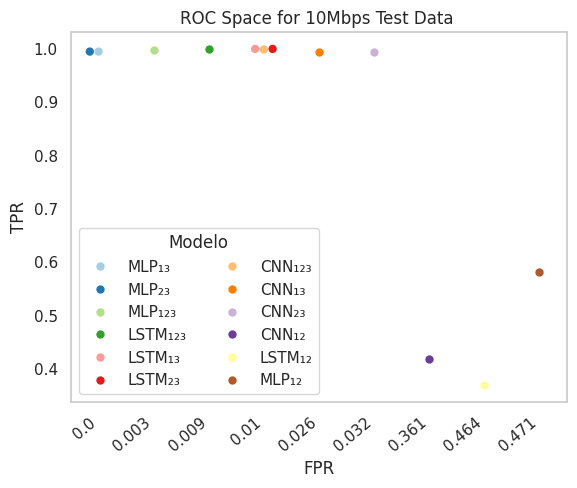
\includegraphics[width=1.0\textwidth]{./figs/ROC-Space-Test-Data-10Mbps.png}
	\captionof{figure}{ROC space test Data 10Mbps.}
	\label{fig:ROCDesempenhoteste10Mbps}	
\end{minipage}
\begin{minipage}{0.1\textwidth}
	\centering
	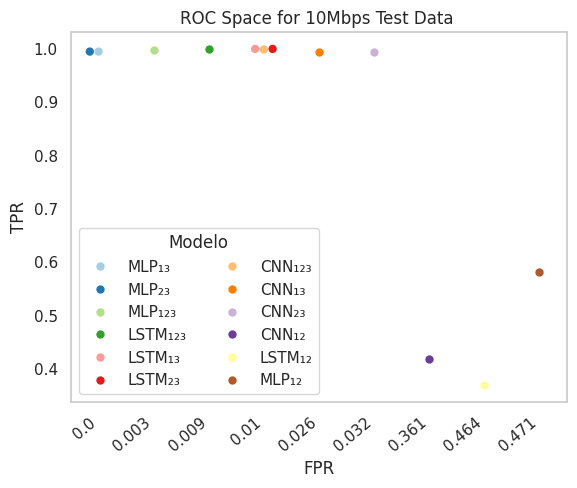
\includegraphics[width=1.0\textwidth]{./figs/ROC-Space-Test-Data-10Mbps.png}
	\captionof{figure}{ROC space test Data 10Mbps.}
	\label{fig:ROCDesempenhoteste10Mbps}	
\end{minipage}
\begin{minipage}{0.1\textwidth}
	\centering
	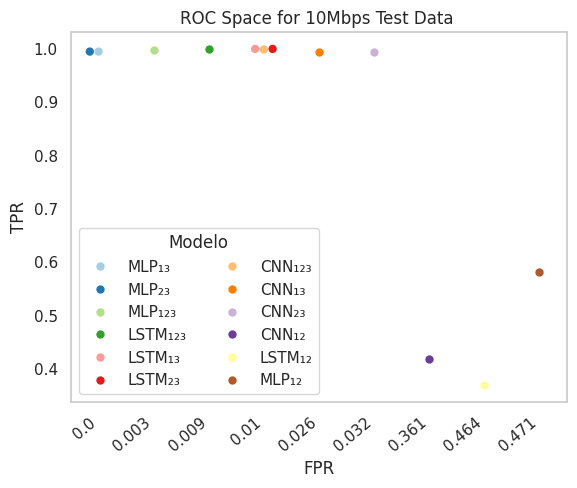
\includegraphics[width=1.0\textwidth]{./figs/ROC-Space-Test-Data-10Mbps.png}
	\captionof{figure}{ROC space test Data 10Mbps.}
	\label{fig:ROCDesempenhoteste10Mbps}	
\end{minipage}
\begin{minipage}{0.1\textwidth}
	\centering
	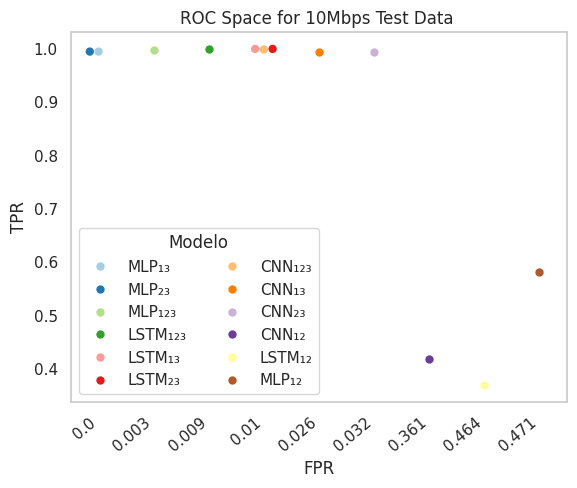
\includegraphics[width=1.0\textwidth]{./figs/ROC-Space-Test-Data-10Mbps.png}
	\captionof{figure}{ROC space test Data 10Mbps.}
	\label{fig:ROCDesempenhoteste10Mbps}	
\end{minipage}
\begin{minipage}{0.1\textwidth}
	\centering
	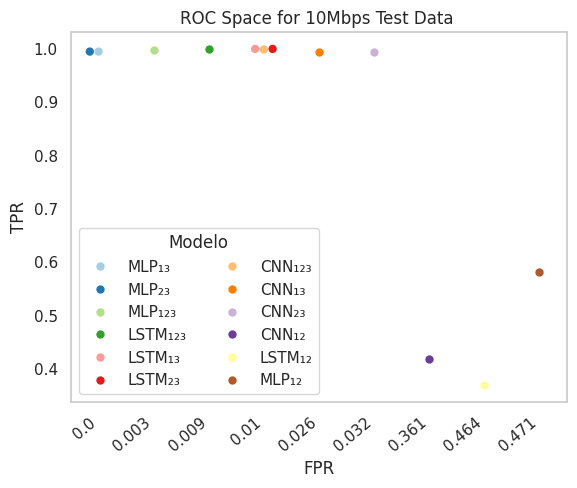
\includegraphics[width=1.0\textwidth]{./figs/ROC-Space-Test-Data-10Mbps.png}
	\captionof{figure}{ROC space test Data 10Mbps.}
	\label{fig:ROCDesempenhoteste10Mbps}	
\end{minipage}
\hfill
\endgroup














\begingroup
\setlength{\tabcolsep}{0.5pt} % Default value: 6pt

\begin{table}
	\centering
	\caption{ROC space and Metrics for 10Mbps bottleneck.}	
	\begin{tabular*}{\textwidth}{@{} CC@{} }
		\hline
		\toprule
		ROC Space & Metrics \\ \hline
		\midrule	
		& \\
		
		\begin{minipage}{0.55\textwidth}
			%\begingroup
			
			%\begin{figure}
			%\vspace{-0.4cm}
			\hspace{0.5cm}
			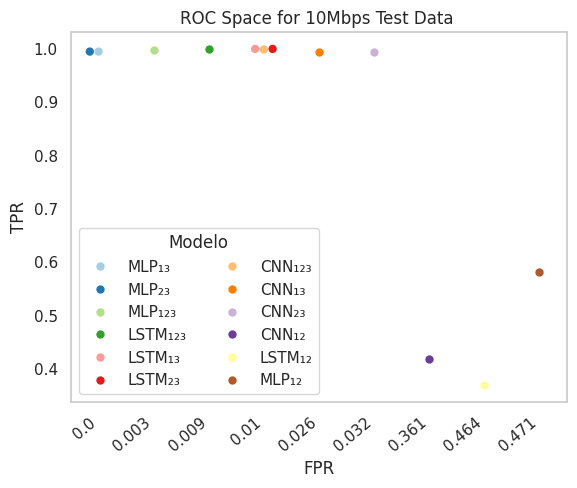
\includegraphics[width=.60\textwidth]{./figs/ROC-Space-Test-Data-10Mbps.png}
			\subcaption{ }
			\label{fig:desempenhoteste}
			%\end{figure}
			%\endgroup
		\end{minipage}
		\hfil
		&
		\begin{minipage}{0.45\textwidth}
			\begingroup
			\begin{tiny}	
				\setlength{\tabcolsep}{3pt}
				\renewcommand{\arraystretch}{1.15}
				%%%%%%%%%%%%%%%%%%%%%%%%%%%%%%%%%%%%%%
				
				
				\begin{tabular*}{\textwidth}{@{} CCCCCC@{} }
					\toprule
					Modelo&Acurácia&Erro&Precisão&Recall&F1 \\
					\midrule
					MLP$_{123}$ & $0.997$ & $0.003$ & $0.997$ & $0.998$ & $0.997$ \\
					MLP$_{13}$ & $0.998$ & $0.002$ & $1.000$ & $0.995$ & $0.998$ \\
					MLP$_{23}$ & $0.998$ & $0.002$ & $1.000$ & $0.995$ & $0.997$ \\
					MLP$_{12}$ & $0.547$ & $0.453$ & $0.388$ & $0.582$ & $0.465$ \\
					LSTM$_{123}$ & $0.994$ & $0.006$ & $0.986$ & $1.000$ & $0.993$ \\
					LSTM$_{13}$ & $0.994$ & $0.006$ & $0.984$ & $1.000$ & $0.992$ \\
					LSTM$_{23}$ & $0.994$ & $0.006$ & $0.985$ & $1.000$ & $0.992$ \\
					LSTM$_{12}$ & $0.418$ & $0.582$ & $0.661$ & $0.370$ & $0.475$ \\
					CNN$_{123}$ & $0.994$ & $0.006$ & $0.985$ & $0.999$ & $0.992$ \\
					CNN$_{13}$ & $0.981$ & $0.019$ & $0.959$ & $0.994$ & $0.976$ \\
					CNN$_{23}$ & $0.978$ & $0.022$ & $0.950$ & $0.994$ & $0.972$ \\
					CNN$_{12}$ & $0.502$ & $0.498$ & $0.658$ & $0.419$ & $0.512$ \\    		
					\bottomrule
				\end{tabular*}
				\subcaption{ }\label{tab:metricas10Mbps}
			\end{tiny}
			\endgroup
			
			%%%%%%%%%%%%%%%%%%%%%%%%%%%%%%%%%%%%%%
			
		\end{minipage}
		\hfil
		\\ \hline
		
		
	\end{tabular*}
	
\end{table}


\begin{table}
	\begin{tabular}{c}
		\\
		\begin{minipage}{0.45\textwidth}
			%%%%%%%%%%%%%%%%%%%%%%%%%%%%%%%%%%%%%%
			\captionof{table}{Model Metrics - 10Mbps}\label{tab:metricas10Mbps}
			\begin{tabular*}{\textwidth}{@{} CCCCCC@{} }
				\toprule
				Modelo&Acurácia&Erro&Precisão&Recall&F1 \\
				\midrule
				MLP$_{123}$ & $0.997$ & $0.003$ & $0.997$ & $0.998$ & $0.997$ \\
				MLP$_{13}$ & $0.998$ & $0.002$ & $1.000$ & $0.995$ & $0.998$ \\
				MLP$_{23}$ & $0.998$ & $0.002$ & $1.000$ & $0.995$ & $0.997$ \\
				MLP$_{12}$ & $0.547$ & $0.453$ & $0.388$ & $0.582$ & $0.465$ \\
				LSTM$_{123}$ & $0.994$ & $0.006$ & $0.986$ & $1.000$ & $0.993$ \\
				LSTM$_{13}$ & $0.994$ & $0.006$ & $0.984$ & $1.000$ & $0.992$ \\
				LSTM$_{23}$ & $0.994$ & $0.006$ & $0.985$ & $1.000$ & $0.992$ \\
				LSTM$_{12}$ & $0.418$ & $0.582$ & $0.661$ & $0.370$ & $0.475$ \\
				CNN$_{123}$ & $0.994$ & $0.006$ & $0.985$ & $0.999$ & $0.992$ \\
				CNN$_{13}$ & $0.981$ & $0.019$ & $0.959$ & $0.994$ & $0.976$ \\
				CNN$_{23}$ & $0.978$ & $0.022$ & $0.950$ & $0.994$ & $0.972$ \\
				CNN$_{12}$ & $0.502$ & $0.498$ & $0.658$ & $0.419$ & $0.512$ \\    		
				\bottomrule
			\end{tabular*}
			
			
			%%%%%%%%%%%%%%%%%%%%%%%%%%%%%%%%%%%%%%
			
		\end{minipage}
		
		\hfill
		\begin{minipage}{0.55\textwidth}
			\centering
			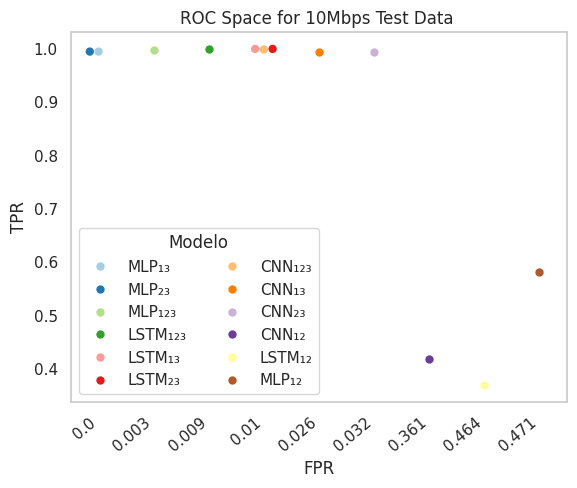
\includegraphics[width=.8\textwidth]{./figs/ROC-Space-Test-Data-10Mbps.png}
			\captionof{figure}{ROC space\\ test Data 10Mbps.}
			\label{fig:desempenhoteste}
			
			
		\end{minipage}
		\hfill
		
		\\
		\bottomrule
	\end{tabular}
	%\caption{Models performance on test data.}
\end{table}


\begin{minipage}{0.45\textwidth}
	\captionof{table}{Desempenho dos modelos sobre os dados de Teste}
	\begin{tabular}{|p{1.5cm}|c|c|c|p{1cm}|c|}
		\hline
		Modelo&Acurácia&Erro&Precisão&Recall&F1 \\
		\hline
		MLP$_{123}$&$0,900$&$0,100$&$0,882$&$0,913$&$0,897$\\ \hline
		MLP$_{13}$&$0,895$&$0,105$&$0,869$&$0,912$&$0,890$\\ \hline
		MLP$_{23}$&$0,876$&$0,124$&\cellcolor{lightgray}{$0,983$}&$0,809$&$0,887$\\ \hline
		MLP$_{12}$&$0,672$&$0,328$&$0,678$&$0,667$&$0,672$\\ \hline
		
		LSTM$_{123}$&$0,891$&$0,109$&$0,854$&$0,921$&$0,886$\\ \hline
		LSTM$_{13}$&$0,878$&$0,122$&$0,872$&$0,869$&$0,871$\\ \hline
		LSTM$_{23}$&$0,862$&$0,138$&$0,907$&$0,828$&$0,866$\\ \hline
		LSTM$_{12}$&$0,695$&$0,305$&$0,717$&$0,676$&$0,696$\\ \hline
		
		CNN$_{123}$&\cellcolor{lightgray}{$0,926$}&\cellcolor{lightgray}{$0,074$}&$0,914$&\cellcolor{lightgray}{$0,931$}&\cellcolor{lightgray}{$0,923$}\\  \hline
		CNN$_{13}$&$0,869$&$0,131$&$0,981$&$0,794$&$0,878$\\ \hline
		CNN$_{23}$&$0,863$&$0,137$&$0,982$&$0,785$&$0,873$\\ \hline
		CNN$_{12}$&$0,670$&$0,330$&$0,638$&$0,681$&$0,659$\\ \hline
	\end{tabular}
	\label{tab:desempenhotestes}
\end{minipage}
\hfill
\begin{minipage}{0.45\textwidth}
	\captionof{table}{Desempenho dos modelos sobre os dados de Teste}
	\begin{tabular}{|p{1.5cm}|c|c|c|p{1cm}|c|}
		\hline
		Modelo&Acurácia&Erro&Precisão&Recall&F1 \\
		\hline
		MLP$_{123}$&$0,900$&$0,100$&$0,882$&$0,913$&$0,897$\\ \hline
		MLP$_{13}$&$0,895$&$0,105$&$0,869$&$0,912$&$0,890$\\ \hline
		MLP$_{23}$&$0,876$&$0,124$&\cellcolor{lightgray}{$0,983$}&$0,809$&$0,887$\\ \hline
		MLP$_{12}$&$0,672$&$0,328$&$0,678$&$0,667$&$0,672$\\ \hline
		
		LSTM$_{123}$&$0,891$&$0,109$&$0,854$&$0,921$&$0,886$\\ \hline
		LSTM$_{13}$&$0,878$&$0,122$&$0,872$&$0,869$&$0,871$\\ \hline
		LSTM$_{23}$&$0,862$&$0,138$&$0,907$&$0,828$&$0,866$\\ \hline
		LSTM$_{12}$&$0,695$&$0,305$&$0,717$&$0,676$&$0,696$\\ \hline
		
		CNN$_{123}$&\cellcolor{lightgray}{$0,926$}&\cellcolor{lightgray}{$0,074$}&$0,914$&\cellcolor{lightgray}{$0,931$}&\cellcolor{lightgray}{$0,923$}\\  \hline
		CNN$_{13}$&$0,869$&$0,131$&$0,981$&$0,794$&$0,878$\\ \hline
		CNN$_{23}$&$0,863$&$0,137$&$0,982$&$0,785$&$0,873$\\ \hline
		CNN$_{12}$&$0,670$&$0,330$&$0,638$&$0,681$&$0,659$\\ \hline
	\end{tabular}
	\label{tab:desempenhotestes}
\end{minipage}
\hfill
\endgroup
